\documentclass[tikz,border=6pt]{standalone}
\usepackage{amsmath,amssymb}
\usepackage[scaled=0.92]{helvet}
\renewcommand{\familydefault}{\sfdefault}
\usepackage{xcolor}
\usetikzlibrary{arrows.meta,positioning,fit,backgrounds,calc,patterns}

% Professional Academic Color Palette (IEEE Systems Style)
\definecolor{edgeshade}{HTML}{2B6CB0}
\definecolor{cloudshade}{HTML}{C05621}
\definecolor{wanshade}{HTML}{64748B}

\definecolor{sparsefill}{HTML}{CCFBF1}
\definecolor{sparsestroke}{HTML}{0D9488}
\definecolor{densefill}{HTML}{DBEAFE}
\definecolor{densestroke}{HTML}{2563EB}

\definecolor{prefillfill}{HTML}{FFEDD5}
\definecolor{prefillstroke}{HTML}{EA580C}
\definecolor{specprefillfill}{HTML}{D1FAE5}
\definecolor{specprefillstroke}{HTML}{059669}

\definecolor{stallfill}{HTML}{F8FAFC}
\definecolor{stallstroke}{HTML}{94A3B8}
\definecolor{textdark}{HTML}{0F172A}
\definecolor{textmuted}{HTML}{475569}

\begin{document}
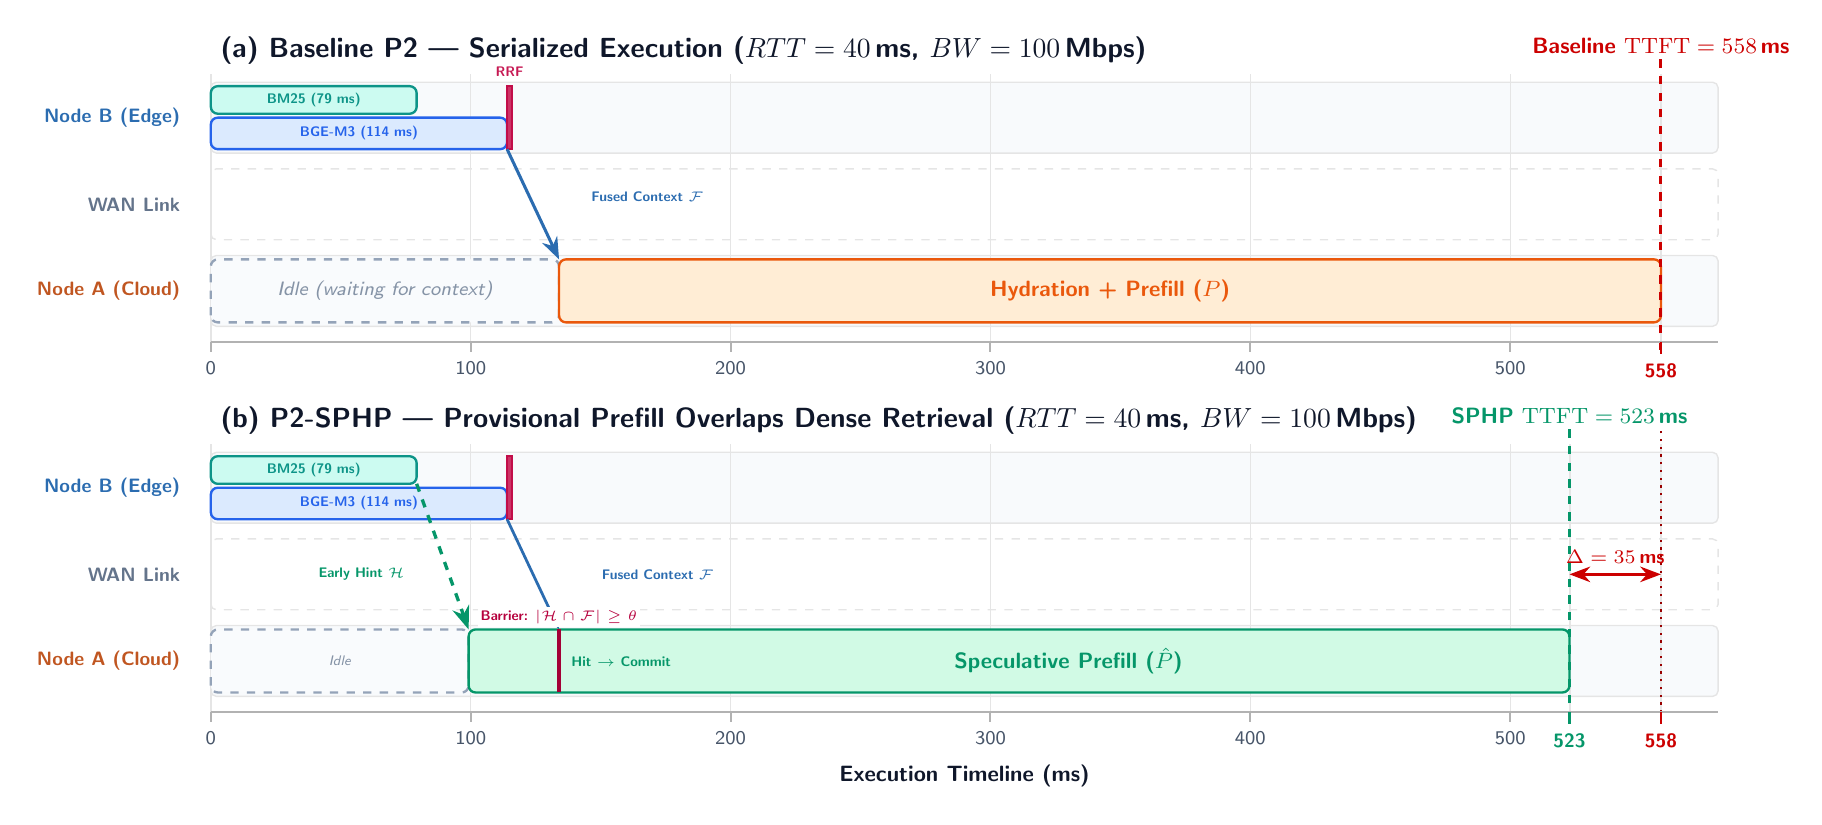
\begin{tikzpicture}[
    font=\small,
    >=Stealth,
    x=0.033cm, y=1.0cm,
    barblock/.style={
        rounded corners=2.5pt,
        line width=0.85pt,
        inner sep=0pt
    }
]

% ===========================================================================
% PANEL (a): BASELINE P2 (SERIALIZED)
% ===========================================================================
\node[anchor=west, font=\bfseries\normalsize, text=textdark] at (0, 8.1) 
    {(a) Baseline P2 --- Serialized Execution ($RTT = 40\,\text{ms}$, $BW = 100\,\text{Mbps}$)};

% Track backgrounds
\draw[fill=stallfill, draw=gray!20, line width=0.5pt, rounded corners=2pt] (0, 6.8) rectangle (580, 7.7); % Node B
\draw[fill=white, draw=gray!20, line width=0.5pt, dashed, rounded corners=2pt] (0, 5.7) rectangle (580, 6.6); % WAN
\draw[fill=stallfill, draw=gray!20, line width=0.5pt, rounded corners=2pt] (0, 4.6) rectangle (580, 5.5); % Node A

% Track labels (left)
\node[anchor=east, font=\scriptsize\bfseries, text=edgeshade] at (-8, 7.25) {Node B (Edge)};
\node[anchor=east, font=\scriptsize\bfseries, text=wanshade]  at (-8, 6.15) {WAN Link};
\node[anchor=east, font=\scriptsize\bfseries, text=cloudshade] at (-8, 5.05) {Node A (Cloud)};

% Grid lines
\foreach \t in {0, 100, 200, 300, 400, 500, 558} {
    \draw[draw=gray!20, line width=0.5pt] (\t, 4.4) -- (\t, 7.8);
}

% --- Execution Blocks on Node B ---
% Sparse Retrieval: 0 to 79.2 ms
\draw[barblock, draw=sparsestroke, fill=sparsefill] (0, 7.3) rectangle (79.2, 7.65);
\node[font=\tiny\bfseries, text=sparsestroke] at (39.6, 7.475) {BM25 (79 ms)};

% Dense Retrieval: 0 to 114.0 ms
\draw[barblock, draw=densestroke, fill=densefill] (0, 6.85) rectangle (114.0, 7.25);
\node[font=\tiny\bfseries, text=densestroke] at (57.0, 7.05) {BGE-M3 (114 ms)};

% RRF Fusion: 114.0 to 116.0 ms
\draw[fill=purple!80, draw=purple!95, line width=0.6pt] (114.0, 6.85) rectangle (116.0, 7.65);
\node[anchor=south, font=\tiny\bfseries, text=purple!90] at (115.0, 7.65) {RRF};

% --- Stalled on Node A ---
\draw[barblock, draw=stallstroke, fill=stallfill!80, dashed] (0, 4.65) rectangle (134.0, 5.45);
\node[font=\scriptsize\itshape, text=stallstroke!90!black] at (67.0, 5.05) {Idle (waiting for context)};

% --- WAN Transfer: 114.0 to 134.0 ms ---
\draw[->, line width=1.1pt, draw=edgeshade] (114.0, 6.85) -- (134.0, 5.45);
\node[font=\tiny\bfseries, text=edgeshade] at (168.0, 6.25) {Fused Context $\mathcal{F}$};

% --- Hydration + Prefill on Node A: 134.0 to 558.0 ms ---
\draw[barblock, draw=prefillstroke, fill=prefillfill] (134.0, 4.65) rectangle (558.0, 5.45);
\node[font=\footnotesize\bfseries, text=prefillstroke] at (346.0, 5.05) 
    {Hydration + Prefill ($P$)};

% --- Baseline TTFT Marker ---
\draw[line width=1.1pt, draw=red!80!black, dashed] (558.0, 4.3) -- (558.0, 8.0);
\node[anchor=south, font=\footnotesize\bfseries, text=red!80!black, fill=white, inner sep=1.5pt] at (558.0, 8.0) 
    {Baseline $\mathrm{TTFT} = 558\,\text{ms}$};

% Timeline Axis (Panel a)
\draw[line width=0.8pt, draw=gray!60] (0, 4.4) -- (580, 4.4);
\foreach \t in {0, 100, 200, 300, 400, 500} {
    \draw[line width=0.7pt, draw=gray!60] (\t, 4.4) -- (\t, 4.28);
    \node[anchor=north, font=\scriptsize, text=textmuted] at (\t, 4.28) {\t};
}
\draw[line width=0.9pt, draw=red!80!black] (558.0, 4.4) -- (558.0, 4.25);
\node[anchor=north, font=\scriptsize\bfseries, text=red!80!black] at (558.0, 4.25) {558};


% ===========================================================================
% PANEL (b): P2-SPHP (SPECULATIVE PREFILL OVERLAP)
% ===========================================================================
\node[anchor=west, font=\bfseries\normalsize, text=textdark] at (0, 3.4) 
    {(b) P2-SPHP --- Provisional Prefill Overlaps Dense Retrieval ($RTT = 40\,\text{ms}$, $BW = 100\,\text{Mbps}$)};

% Track backgrounds
\draw[fill=stallfill, draw=gray!20, line width=0.5pt, rounded corners=2pt] (0, 2.1) rectangle (580, 3.0); % Node B
\draw[fill=white, draw=gray!20, line width=0.5pt, dashed, rounded corners=2pt] (0, 1.0) rectangle (580, 1.9); % WAN
\draw[fill=stallfill, draw=gray!20, line width=0.5pt, rounded corners=2pt] (0, -0.1) rectangle (580, 0.8); % Node A

% Track labels (left)
\node[anchor=east, font=\scriptsize\bfseries, text=edgeshade] at (-8, 2.55) {Node B (Edge)};
\node[anchor=east, font=\scriptsize\bfseries, text=wanshade]  at (-8, 1.45) {WAN Link};
\node[anchor=east, font=\scriptsize\bfseries, text=cloudshade] at (-8, 0.35) {Node A (Cloud)};

% Grid lines
\foreach \t in {0, 100, 200, 300, 400, 500, 523, 558} {
    \draw[draw=gray!20, line width=0.5pt] (\t, -0.3) -- (\t, 3.1);
}

% --- Execution Blocks on Node B ---
% Sparse Retrieval: 0 to 79.2 ms
\draw[barblock, draw=sparsestroke, fill=sparsefill] (0, 2.6) rectangle (79.2, 2.95);
\node[font=\tiny\bfseries, text=sparsestroke] at (39.6, 2.775) {BM25 (79 ms)};

% Dense Retrieval: 0 to 114.0 ms
\draw[barblock, draw=densestroke, fill=densefill] (0, 2.15) rectangle (114.0, 2.55);
\node[font=\tiny\bfseries, text=densestroke] at (57.0, 2.35) {BGE-M3 (114 ms)};

% RRF Fusion: 114.0 to 116.0 ms
\draw[fill=purple!80, draw=purple!95, line width=0.6pt] (114.0, 2.15) rectangle (116.0, 2.95);

% --- FLOW 1: Speculative Hint Stream @ 79.2 ms ---
\draw[->, dashed, line width=1.2pt, draw=specprefillstroke] (79.2, 2.6) -- (99.2, 0.75);
\node[font=\tiny\bfseries, text=specprefillstroke] at (58.0, 1.45) {Early Hint $\mathcal{H}$};

% --- FLOW 2: Fused Context Stream @ 114.0 ms ---
\draw[->, line width=1.0pt, draw=edgeshade] (114.0, 2.15) -- (134.0, 0.75);
\node[font=\tiny\bfseries, text=edgeshade] at (172.0, 1.45) {Fused Context $\mathcal{F}$};

% --- Node A Idle: 0 to 99.2 ms ---
\draw[barblock, draw=stallstroke, fill=stallfill!80, dashed] (0, -0.05) rectangle (99.2, 0.75);
\node[font=\tiny\itshape, text=stallstroke!90!black] at (49.6, 0.35) {Idle};

% --- Speculative Prefill on Node A: 99.2 to 522.8 ms ---
\draw[barblock, draw=specprefillstroke, fill=specprefillfill] (99.2, -0.05) rectangle (522.8, 0.75);
\node[font=\footnotesize\bfseries, text=specprefillstroke] at (330.0, 0.35) 
    {Speculative Prefill ($\hat{P}$)};

% Verification Gate barrier at 134.0 ms
\draw[line width=1.3pt, draw=purple!85!black] (134.0, -0.05) -- (134.0, 0.75);
\node[anchor=south, font=\tiny\bfseries, text=purple!95!black, fill=white, inner sep=1pt] at (134.0, 0.78) 
    {Barrier: $|\mathcal{H} \cap \mathcal{F}| \ge \theta$};
\node[anchor=south west, font=\tiny\bfseries, text=specprefillstroke] at (135.0, 0.15) 
    {Hit $\to$ Commit};

% --- SPHP TTFT Marker ---
\draw[line width=1.1pt, draw=specprefillstroke, dashed] (522.8, -0.4) -- (522.8, 3.3);
\node[anchor=south, font=\footnotesize\bfseries, text=specprefillstroke, fill=white, inner sep=1.5pt] at (522.8, 3.3) 
    {SPHP $\mathrm{TTFT} = 523\,\text{ms}$};

% Baseline reference line
\draw[line width=0.8pt, draw=red!60!black, dotted] (558.0, -0.4) -- (558.0, 3.3);

% Latency Delta Bracket: 522.8 to 558.0 ms
\draw[<->, line width=1.0pt, draw=red!80!black] (522.8, 1.45) -- node[above, font=\scriptsize\bfseries, text=red!80!black] {$\Delta = 35\,\text{ms}$} (558.0, 1.45);

% Timeline Axis (Panel b)
\draw[line width=0.8pt, draw=gray!60] (0, -0.3) -- (580, -0.3);
\foreach \t in {0, 100, 200, 300, 400, 500} {
    \draw[line width=0.7pt, draw=gray!60] (\t, -0.3) -- (\t, -0.42);
    \node[anchor=north, font=\scriptsize, text=textmuted] at (\t, -0.42) {\t};
}
\draw[line width=0.9pt, draw=specprefillstroke] (522.8, -0.3) -- (522.8, -0.45);
\node[anchor=north, font=\scriptsize\bfseries, text=specprefillstroke] at (522.8, -0.45) {523};

\draw[line width=0.9pt, draw=red!80!black] (558.0, -0.3) -- (558.0, -0.45);
\node[anchor=north, font=\scriptsize\bfseries, text=red!80!black] at (558.0, -0.45) {558};

\node[anchor=north, font=\footnotesize\bfseries, text=textdark] at (290, -0.85) {Execution Timeline (ms)};

\end{tikzpicture}
\end{document}
